\documentclass[a4paper,12pt]{article}
% Use the options 'crop' to show crop marks, and
% 'doublespaced' for double line spacing.
% e.g. \documentclass[crop,doublespaced]{cupjournal}


%calling packages
\usepackage[english]{babel}
\usepackage[utf8]{inputenc}
\usepackage{amsmath}
\usepackage{graphicx}
\usepackage[left=1in,right=1in,top=1in,bottom=1in]{geometry}
\usepackage{setspace}
\usepackage[round]{natbib}
\usepackage{epstopdf}
\usepackage{soul}
\usepackage{lmodern}
\usepackage{caption}
\usepackage{hyperref}
\usepackage{subcaption}
\usepackage{rotating}
%\usepackage{etoc}


\usepackage{xr}
\externaldocument{"appendix"}


\usepackage{longtable}
\usepackage{amssymb}
\usepackage{fancyhdr}
\usepackage{array}
\usepackage{lscape} % for landscape formatting of pages
\newcolumntype{P}[1]{>{\centering\arraybackslash}p{#1}}
%fonts
\usepackage{times}
%\setcounter{secnumdepth}{0}
%chanfing font of table headers
\captionsetup[figure]{labelfont=bf}
\captionsetup[table]{labelfont=bf}

%path to where figures are located
\graphicspath{ {images/} }

%for notes in table captions 
\newcommand\fnote[1]{\captionsetup{font=small}\caption*{#1}}

%changing header
\pagestyle{fancy}
\fancyhf{}
\rhead{\thepage}
\renewcommand{\headrulewidth}{0pt}
\renewcommand{\footrulewidth}{0pt}
\renewcommand*\footnoterule{}
\let\svfootnoterule\footnoterule
\renewcommand\footnoterule{\vspace{0.2in}\svfootnoterule}
\renewcommand*{\thefootnote}{\fnsymbol{footnote}}
%set spacing

\renewcommand{\sfdefault}{phv}

\doublespacing
\usepackage{titlesec}

\titleformat*{\section}{\Large\sffamily}
\titleformat*{\subsection}{\large\sffamily}
\titlespacing*\section{0pt}{24pt plus 4pt minus 2pt}{4pt plus 2pt minus 2pt}
\titlespacing*\subsection{0pt}{20pt plus 4pt minus 2pt}{4pt plus 2pt minus 2pt}


%changing title settings
\makeatletter
\renewcommand{\maketitle}{
	\begin{flushleft}
		
		\onehalfspacing
		
		\@title
		
		\lineskip .5em
		\normalfont{\normalsize{\@author}}
\end{flushleft}}
\makeatother


\newcommand{\beginsupplement}{%
	\setcounter{table}{0}
	\renewcommand{\thetable}{S.\arabic{table}}%
	\setcounter{figure}{0}
	\renewcommand{\thefigure}{S.\arabic{figure}}%
}


%title
\title{\bigskip \bigskip \sffamily \LARGE{Can Citizens Set City Policy?} \\ \Large{ Evidence From A Decentralized Welfare State}}

%author
\author{\bigskip Benjamin Carl Egerod\footnote[2]{Graduate Student, Department of Political Science, University of Copenhagen, e-mail: \texttt{benjamin.carl.egerod@ifs.ku.dk}.} \qquad Martin Vinæs Larsen\footnote[3]{Assistant Professor, Department of Political Science, Aarhus University, e-mail: \texttt{mvl@ps.au.dk}.}} 



\begin{document}

	
	\begin{footnotesize} \noindent \today. \end{footnotesize} %date
	
	\vspace{0.7in}
	
	\maketitle
	
	\bigskip
	
	\begin{quotation} %abstract

		\small \noindent \emph{Abstract:} Municipal governments supposedly empower citizens, giving them the ability to shape the political organization of their local community. In spite of this, we know little about whether municipal governments are in fact responsive to the policy views of municipal electorates. In this study, we look at whether the policy implemented by local politicians actually respond to changes in the public mood. To do this, we compile a unique and comprehensive dataset of local fiscal policy, which we use to construct municipal-level estimates of fiscal policy conservatism. This detailed policy data is then linked to an indicator of local ideological sentiment. We find strong evidence for dynamic responsiveness: when preferences in a municipality changes, public policy responds.
	\end{quotation}



	
	\thispagestyle{empty} %removing page number from page one
	
	
\clearpage


\noindent In most developed countries municipal governments are an essential part of representative government \citep{trounstine2009all,kersting2013reforming}. They are responsible for a large part of public spending.  They are able to levy taxes on income and property. And while they are subordinate to central governments, oversight is always limited in formal or informal ways \citep{oecd2016subnational}. Municipalities thus play a central part in the quintessential political act of deciding who gets what, when and how. From the standpoint of democratic representation it is important to ask whether citizens are able to set set policy? Or whether policy is set for them by extraneous forces?

%Skiftet 'interesting' til 'important'

There are good reasons to be skeptical of municipal governments' democratic potential, as  several forces limit municipal governments capacity to respond to public concerns. Central governments often put constraints on local government decision-making \citep{peterson1981city}. Similarly, competition with other adjacent municipalities might restrain policy-making \citep{salmon2006horizontal,tiebout1956pure}. Furthermore, Even if municipalities have the capacity to set policy independently, voters might not be able to effectively influence policy-making \citep[e.g.,][]{sances2017attribution,gerber2011mayors}. 

%neden for har jeg slettet 'as such' før 'voters tend to'. Og jeg har erstattet det andet 'voters tend to' med et 'and'. Tænker, det henviser tilbage til den første forekomst af 'voters'.

Recent empirical studies of municipal government, however, suggest that such concerns might not be warranted. Voters tend to (re-)elect local politicians based on their actions in office \citep{arnold2012holding,burnett2017politics,boyne2009democracy}, and to vote for conservative (liberal)  mayors if they themselves hold conservative (liberal) policy views  \citep{sances2017ideology,boudreau2015lost,hopkins2017retrospective}. Furthermore, a number of studies have found that it matters for city policy whether a conservative or a liberal party controls the mayoralty and/or the city council \citep{fiva2016power,folke2014shades,blom2006parties,de2016mayoral}. 

% neden for har jeg slettet to detaljer om studierne: "using a lagged dependent variable approach" og "In an unpublished study,"

While these studies provide \textit{indirect} evidence that municipalities are responsive, there are only a few studies that examine municipal responsiveness more directly. Most notably, Tausanovitch and Warshaw use Multilevel Regression with Poststratification (MRP) to estimate the policy preferences of citizens in a cross section of US cities. They find a strong and robust correlation between these preferences and city policy \citep[for earlier efforts, see ][]{hajnal2010or,palus2010responsiveness}. Since then, two other studies have directly examined municipal responsiveness. The first of these are \cite{einstein2016pushing}. Here, the authors also identify a strong correlation between citizen preferences, measured as support for the Democratic party at presidential elections,  and city policy. Apart from replicating the findings from \citeauthor{tausanovitch2014representation}, \citeauthor{einstein2016pushing} are also able to identify the use of intergovernmental grants as a key mechanism underlying responsiveness. They also offer a stronger identification strategy by examining responsiveness in a panel of cities from two US states.  \citet{sances2017voters} expands on existing work using a panel of 3,000 US counties spanning 50 years. Linking changes in Democratic vote share to county-level policy, Sances finds that as counties grow more Democratic they tend to spend more and to collect more own-source revenues.

% neden for erstatter jeg "also puts limits on what" med "also limits"
% Jeg er usikker på følgende sætning: "In particular, it is hard to know whether municipal policy respond to changes in policy. That is, whether municipal policy is dynamically responsive." Den første del kan lyde som et spørgsmål om kausalinferens, men det er ikke den pointe, vi gerne vil lave her - er usikker på, hvordan det ellers kan formuleres.
All in all, research in the area of municipal responsiveness has made impressive progress in the past few years. However, the existing evidence remains limited in important ways. First, city policy is usually measured using either few indicators \citep{sances2017voters,einstein2016pushing} or at a single point in time \citep{tausanovitch2014representation}. Relatedly, previous analyses are either cross-sectional or look at concurrent changes in policy and preferences. This is in part a methodological problem, as the risk of reverse causation looms large when we measure policy and preferences at the same time. However, the static analysis which permeates most of the existing literature also limits the theoretical inferences we can make about responsiveness. In particular, it is hard to know whether municipal policy respond to changes in policy. That is, whether municipal policy is dynamically responsive \citep{stimson1995dynamic}. Finally, the existing literature is exclusively US based, which naturally raises concerns about generalisability.

%neden for har jeg erstattet "we are able to look at" med "we look at".

In this study, we address these limitations related to context, design and data by studying (dynamic) responsiveness in Danish municipalities. In particular, we develop an annual measure of municipal policy conservatism based on 14 fiscal policy indicators (1978-2006). A measure which is much more comprehensive in terms of its granularity, and the time period covered, than the city policy measures used in previous studies. Similar to previous studies, we use net support for conservative (right-wing) parties as a proxy for policy views, but unlike previous studies, which had to rely on electoral support measured at national or regional elections, we look at electoral support at \textit{local} elections dating back to 1970. 

Using this comprehensive dataset, we link past changes in preferencs to future changes in policy to avoid concerns about reverse causality. We find that changes in the policy preferences of citizens are robustly related to changes in city policy. We also show that there is no evidence of reverse causality---i.e., past changes in policy do not predict future changes in preferences---and that the effects of a change in preferences from one election to another are detectable up to nine years later. Our findings thus suggest that citizens, at least partially, set city policy.

%Section on contributions? Maybe 100 words.


\section*{Empirical Strategy}

 We examine municipal responsiveness in Denmark. Denmark is a decentralized welfare state where municipalities can affect their local revenue and set a yearly budget.  Municipal tasks and services include the core welfare services of the Danish welfare state and municipal spending amounts to 35 percent of GDP, which is more than half of all public spending. We focus on Denmark, as this allows us to track the relationship between citizen preferences and city policy in a dynamic way. As such, we are able to get a detailed measure of city policy for all years between 1978 and 2005 for all 271 Danish municipalities.  We can link this to preferences as expressed for right and left wing parties in municipal elections in the same period.
 
 

Danish municipalities are different from the US counties and cities which have been the focus of previous studies. They are small (average size 16,000 inhabitants), organized in general rather than special purpose governments \citep{berry2009imperfect}, with a multi party, PR system where turnout is relatively high.\footnote{See Appendix \ref{context} for more details on the political system in Danish municipalities.} It is not clear whether Denmark is an easy or hard case for responsiveness.  Some factors--such as the small size of the municipalities--seem to make responsiveness less likely than in the US, whereas others--such as the general purpose organization of local government--seem to make responsiveness more likely. As such, the Danish case can not be seen as especially typical or atypical. What makes the Danish case interesting is the high quality data on municipal policy and municipal policy preferences which are available, and the fact that it is a very different setting from the ones previously examined.

%  Unlike most previous research, we do not have to infer that voters preferences for progressive policies are the same at the national and the local level \citep[for an exception, see][]{tausanovitch2014representation}. 

\subsection*{An Annual Measure of Municipal Fiscal Policy Conservatism}

To measure fiscal policy conservatism in Danish municipalities we rely on 14 different indicators relating to either tax policy (3 indicators), spending policy (2), organization of public service delivery (3), co-payment for public services (4) or the extent of public services (2). Variables measured in DKKs are adjusted for inflation. While  spending and tax variables are commonly used in the literature, we are the first to include other types of variables in a panel set-up. An overview of the policy indicators are presented in Appendix \ref{policy}

% Neden for: Er 2016 virkelig endekriteriet og ikke 2006?????

The included policies had to meet the following criteria: (1) The policy should be directly set by the city council.\footnote{It was included even if it was set in collaboration between the city council and some other (set of) actor(s).} (2) It had to be a policy and not the outcome of a policy (i.e., we did not include unemployment). (3) Data on the policy had to be available for at least five years between 1978 and 2016. All policy information was retrieved from Statistics Denmark or the Danish Ministry for Economic Affairs and the Interior.

% Neden for: har slettet at vi automatisk får usikkerhed med, da vi ikke bruger det til noget. Har desuden forsøgt at skrive det mere kompakt og slette gentagne omtale om missingness.

We combine these 14 indicators into an index of fiscal policy conservatism. Inspired by \citeauthor{caughey2016dynamics}s' (2016) analysis of US states, we use a Bayesian latent variable technique to estimate municipal fiscal conservatism as an underlying trait driving municipal policies.  This method is in many ways similar to frequentist factor analysis. However, a major advantage to using Bayesian techniques when making inferences about the latent trait is that the simulations will impute missing data during the estimation, which allows us to include items with different numbers of observations in the model . Using such a technique is particularly important in this case, because data on most indicators is only available after 1993. However, because we use this measurement method, they still shape our estimates of municipal fiscal policy conservatism across the entire period -- the units with missing observations simply supply less information to the estimation. Accordingly, our measure of fiscal policy conservatism for the period 1978-1992 primarily relies on the measures of income tax, property tax and spending pr. capita. To make sure that our results are not driven by the inclusion of different items at different points in time, we perform analyses using only these three variables (reduced measure) as well as with all indicators (full measure). Details about the measurement model can be found in Appendix \ref{estimation}, and in Appendix \ref{descriptives}, we show how municipal policy conservatism varies across time and place in Denmark.

This annual measure of fiscal policy conservatism is more granular and more comprehensive than the indicators of municipal policy used in previous studies. As such, these studies have had to rely on municipal policy measured at one point in time \citep{tausanovitch2014representation,palus2010responsiveness} or measured with substantial intervals\citep{sances2017voters,einstein2016pushing,hajnal2010or}. 



\subsection*{Municipal Policy Preferences}

In order to find out whether municipal fiscal policy conservatism responds to the preferences of the electorate, we need to develop a measure of local policy preferences. In line with previous work on municipal responsiveness \cite[e.g.,][]{sances2017ideology,einstein2016pushing}, we measure local policy preferences indirectly by examining the net difference in electoral support for right-wing and left-wing parties in the municipality, inferring that municipal electorates which prefer conservative parties also prefer conservative fiscal policies. In particular, we look at the difference between support for the major center-right parties as well as the right wing populist parties (Venstre, Det Konservative Folkeparti, Fremskridstpartiet and Dansk Folkeparti) and the major center-left parties as well as the socialist parties (Socialdemokratiet, Radikale Venstre, Socialistisk Folkeparti, Venstresocialisterne, and Enhedslisten) at all municipal elections in the period under study. This gives us an estimate of local policy preferences in the years 1974, 1978, 1981, 1985, 1989, 1993, 1997 and 2001.

 Unlike previous studies, which have had to rely on support for conservative vis-a-vis liberal parties at national or regional elections \citep[e.g.,][]{hajnal2010or,einstein2016pushing}, we are able to look at support at municipal elections. This is potentially important, as citizens might differ in their policy views across domains \cite[for an argument along these lines, see]{abrams2012big}, and because the electorate at municipal elections are differently composed than electorates in national elections \citep{ansolabehere2015beyond,hansen2017social}. In Appendix  \ref{validation} we show that there is added value in using municipal rather than national election returns. In particular, we find that in a concurrent municipal and national election net support for conservative parties is far from perfectly correlated (Pearsons R=0.56).
 
 It might have been preferable to have survey based estimates of citizens policy ideal points \citep[similar to the measure used by][]{tausanovitch2014representation}. However, doing so is not feasible, as survey data is too sparse, especially for the earlier part of the period we study. Instead, we do a validation of our measure in Appendix \ref{validation}, where we show that there is a strong correlation between net support for conservative parties at municipal elections and citizens' responses to an ideology question, using some recent survey data.


\section*{Identifying Dynamic Responsiveness in Cities}

% jeg foreslår, at vi ændrer "asymmetry" til non-linearity. Det kan godt være, at det første er bedre, men jeg er ikke helt sikker på, hvad det ville betyde i sammenhængen.
Figure \ref{fig:scatter} shows that the past changes in support for right-wing parties are related to future changes in fiscal conservatism (full measure), suggesting that  policy adjusts dynamically to changes in preferences. This is striking, as we have minimized concerns related to reverse causality by looking at the relationship between past changes in preferences and future changes in policy -- that is within-municipality. Interestingly, we identify a non-linearity, but this pattern is not robust to alternative specifications (i.e., it disappears in a twoway fixed effects model), so we do not want to make any firm interpretations of what this means.


% neden for står der 10 to gange -- går ud fra, at det er 100 anden gang, men ville ikke ændre det, hvis det viste sig at være forkert
% har markeret med fed i caption.

\begin{figure}[h]
	\centering
	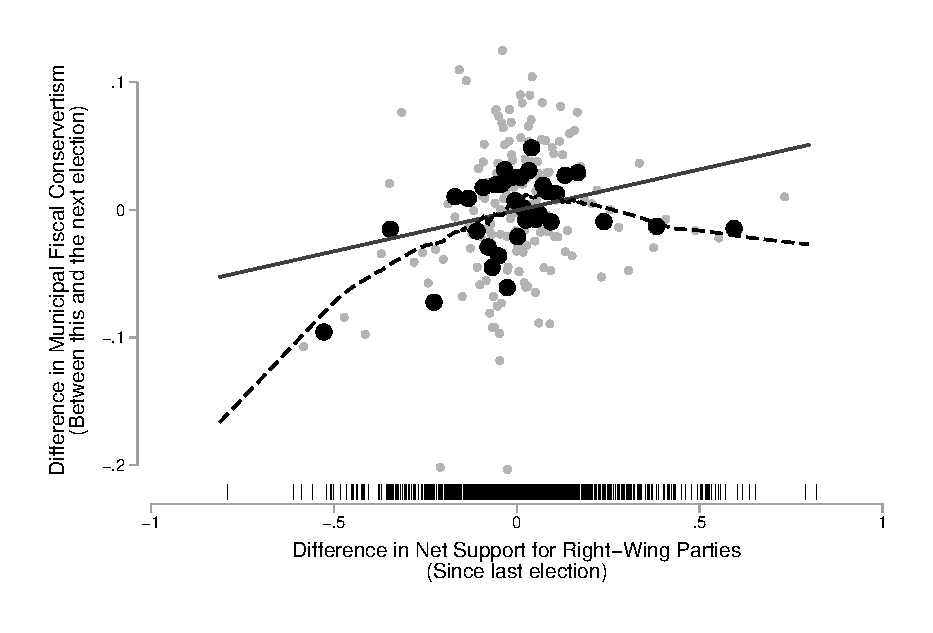
\includegraphics[scale = 0.8]{scatterplot.eps}
	\caption{Do Changes in Preferences Correlate with Future Changes in Policy? Both variables are trend adjusted (i.e., the year specific means are subtracted). Grey dots represent bins of \textbf{ten observations}, dark dots represent bins of \textbf{10} observations. The solid line is a linear fit (b$=0.046$,municipality clustured se$=0.019$) and the dashed line is a LOWESS smoother with a bandwidth of 0.4. The rugplot in the bottom of the graph represents the density of differences in the net proportion voting for right-wing parties variable. }
	\label{fig:scatter}
\end{figure}

\begin{figure}[htbp]
	\centering
	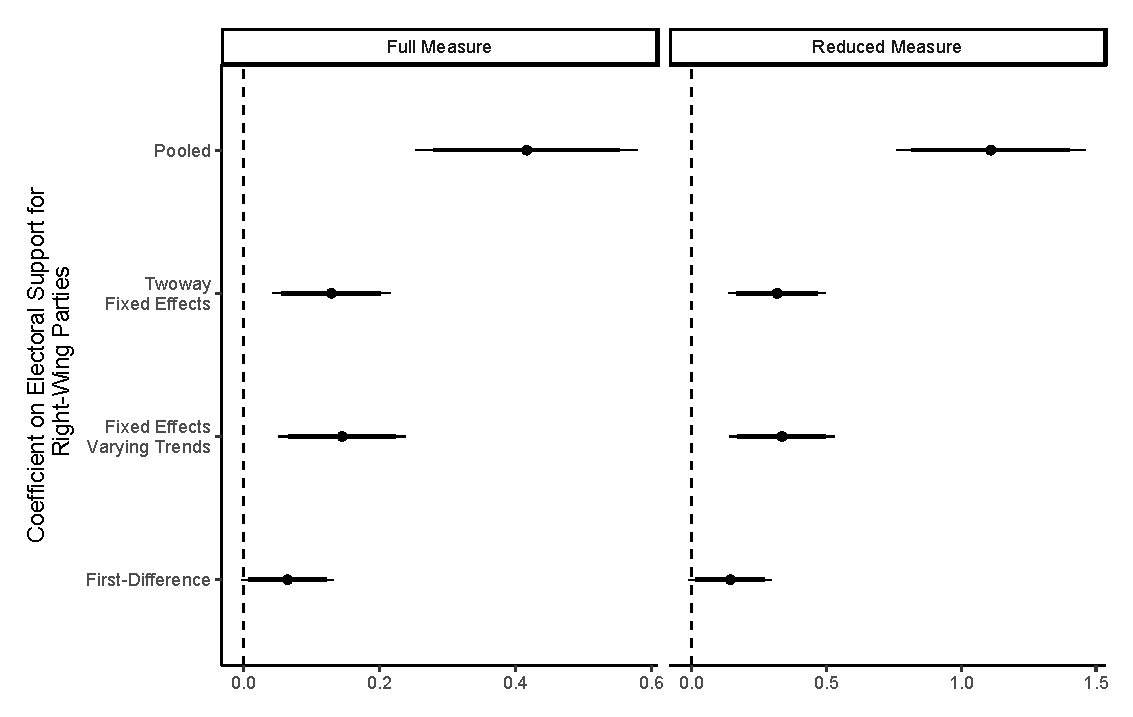
\includegraphics[scale = 0.7]{CoefPlot_18092018.eps}
	\caption{Effect of Electoral Support for Right-wing Parties on Municipal Conservatism 4 years later. Points are unstandardized OLS coefficients. Lines are 95 percent (thin) and 90 percent (thick) confidence intervals (CIs). Beck-Katz standard errors used in first-difference models, Arellano-White standard errors with clustering on municipality level used in the remaining models to correct for temporal autocorrelation. Differences in the coefficients are driven by a larger standard deviation in the reduced measure.}
	\label{fig:FourYearLead}
\end{figure}

%foreslår vi sletter lidt af fedtet her. Har skåret det med "We model this relationship formally ..." fra.
% har desuden forsøgt at frame forskellen mellem pooled- og within-estimater som den deconfoundende effect at at fjerne sociodemografi

Figure \ref{fig:FourYearLead} plots the key estimate (i.e., the effect of changes in local policy preferences) from a pooled OLS regression, as well as from two types of difference-in-differences (diff-in-diff) models: a fixed effects and first-difference model (both with time fixed effects). All models include a control for population size (logged), but the results do not depend on this covariate.  The  left panel uses the full measure of fiscal conservatism as the dependent variable whereas the right panel uses our reduced measure. Across all models we find a statistically significant and positive effect. 

% har slettet: "If we only look at within municipality variation in policy conservatism," og erstattet det med slet og ret "within municipality standard deviation"
Notably, the estimate from the pooled model is likely to be confounded by the socio-demographic make-up of the municipality. To the extent that this is stable over time and driven by common shocks, the difference between the estimates from the pooled and diff-in-diff models can be interpreted as removing the confounding effect of sticky socio-demographics. In our preferred fixed effects model, we estimate the effect to be roughly .12. This corresponds to 25 percent of a within-municipality standard deviation -- a very substantive association. With an effect of this magnitude, moving the voters from the Social Democratic stronghold Albertslund to the highly conservative Gentofte would transform the fiscal policy in Gentofte to roughly that of Sønderborg. This would move Gentofte down by more than 34 positions (out of 271 municipalities) in our ranking of fiscal conservatism.


\subsection*{Exploring the Identifying Assumption}
The identifying assumption in the twoway fixed effects model, is that trends in the dependent variable (policy) are independent of selection into the independent variable (preferences). If municipalities that experience changes in support for right-wing parties already were following different trends in policy this could bias our results. 

While we cannot test the identifying parallel trends assumption directly, we can see whether trends in the dependent are similar before municipalities "select into" different preferences. Importantly, if voters became \emph{more conservative} as a result of changes in policy \cite[cf.][]{lenz2013follow,slothuus2010can}, then we would expect pre-trends to be different. However, if we regress past levels of policy conservatism on current levels of net support for conservative parties using our two-way fixed effect set-up, the effect is negligible and statistically insignificant (see Figure \ref{fig:LongRun}). To  bolster this analysis further,  we show in Appendix \ref{granger} that changes in municipal policy do not precede changes in electoral support for right-wing parties.

% understreger neden for hvor lidt estimatet ændrer sig med interaktion med tidsdummies.
Beyond this indirect test,  we interact the time fixed effects with a series of 13 regional dummies\footnote{These correspond to  13 regional governments (amter) which were responsible for, among other things, health care in the period we study.} as well as population size. This allows municipalities to be on separate time trends depending on both region (semi-parametrically) and population size (log-linearly). Importantly, this strategy should also deal with the confounding effect of the socio-demographic make-up of the municipalities: If there were certain time-specific regional shocks to, for instance, unemployment, which might affect both preferences and policy, then these will be controlled for in this model. As can be seen from Figure \ref{fig:FourYearLead}, it is striking how little estimating this more restrictive model changes our results -- the point estimate increases with XX percent.

To make sure that there is no remaining bias due to these factors, we include data on education, unemployment rate and the number of non-western immigrants in the municipality. Since these variables are only available after 1993, and there is a substantial trend in municipal policy (cf. Appendix \ref{descriptives}), including them would bias our results by censoring the dependent variable. Instead, we follow \citep{pei2018poorly} and regress electoral support for right-wing parties on our three socio-demographic predictors. As we show in Appendix \ref{balance}, the correlations between within-municipality changes in socio-demographic factors and support for right-wing parties are very small and statistically insignificant. This suggests that these important socio-demographic factors are not driving our results. The absence of a correlation with unemployment is especially noteworthy, as it is a strong indicator of whether the municipality is hit particularly hard by a temporary economic shock, which might drive both preferences and policy.

Taken together, these auxiliary analyses suggest that our identifying assumption is met, and thus that we have a good estimate of the effect of municipal policy preferences on municipal policy.

\subsection*{How Dynamic is Dynamic Responsiveness?}

To examine the temporal dynamics of responsiveness, figure \ref{fig:LongRun} reports the estimated effect of changes in net support for conservative parties on  municipal fiscal policy conservatism over time.

\begin{figure}[htbp]
	\centering
	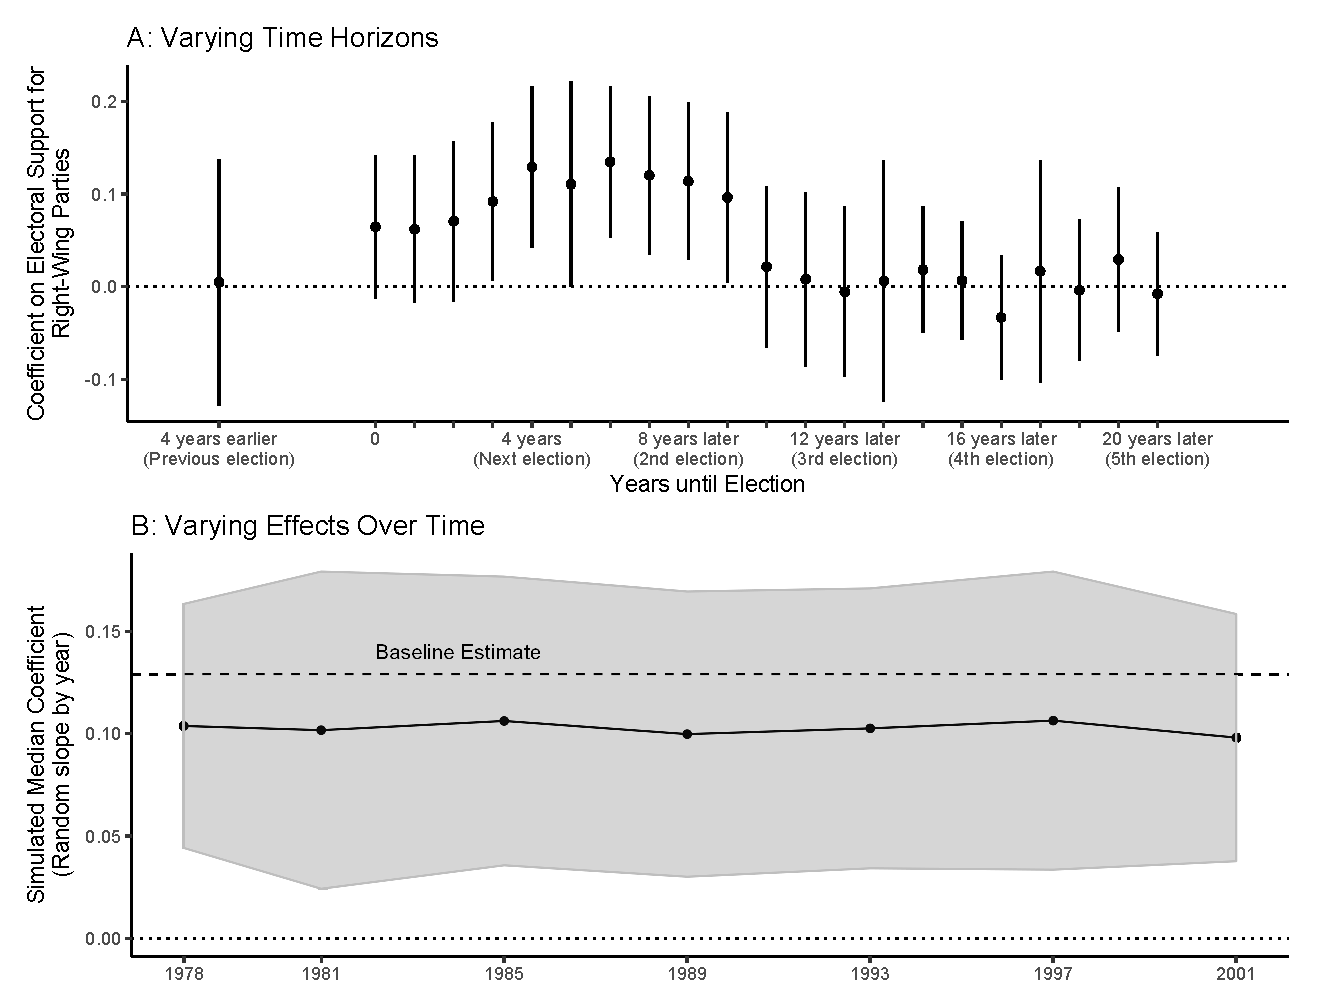
\includegraphics[scale = .6]{EffectsVsTime.eps}
	\caption{Effects of Local Policy Preferences Over Time. All models are twoway fixed effects with control for population size. Panel A: Black points represent the effect of net electoral support for conservative parties with different leads. Black lines are 95 percent CIs based on Arellano-White robust standard errors clustered on municipalities. Panel B: Points are estimates of random slopes by year with a lagged dependent variable to deal with autocorrelation. Shaded area is a 95 percent CI from the relevant percentiles of a bootstrapped distribution of 100 resamples.}
	\label{fig:LongRun}
\end{figure}

In panel A we look at the short and long run effects of changes in municipal policy preferences on the policy adopted by the municipality. This analysis reveals that it takes some time for policy to respond. There is only a small effect one year after local policy preferences change and the largest effect is after four years. The effect is detactable up to eight years later. One reason for this long-term effect is probably that once policy shifts, it typically does not revert back \citep[see, theories of punctuated equilibria, e.g.,][]{baumgartner2009punctuated}.

In Panel B we allow the effect of voter preferences on policy four years into the future to vary through time by including random slopes by year. The results show that municipal policy responsiveness is relatively stable across our period of study. Preferences do not matter more or less as time goes by.




\section*{Conclusion}

In this study, we have shown that municipal government is dynamically responsive to demands from citizens -- when more citizens express that they want more right wing policy, by voting for more right-wing politicians, policy responds. A result that was robust to a number of demanding specifications. Importantly, by using a more detailed and comprehensive measure of municipal policy, we were able to link past changes in preferences to future changes in policy, sidestepping potential concerns related to reverse causality. 

Even so, there are several outstanding questions. For one, we know little about why municipalities respond to citizen preferences. In Appendix \ref{mechanism} we present some evidence to suggest that the effect is not mediated by which party controls the municipal administration, however, this evidence is far from conclusive. Further, while we identify a decent amount of dynamic responsiveness, it is hard to say whether this is a lot or a little from a normative democratic perspective.

Our study contributes directly to the literature on responsiveness, and more broadly the empirical study of whether voters are able constrain the decision-making of political elites. In particular, our study suggests that if you give voters an opportunity to express their preferences at local elections, they are able to use it to direct policy, potentially constraining local policy-makers.





\onehalfspacing
\bibliographystyle{apa}
\bibliography{bibtex/library_NoMiddle}

\clearpage

\renewcommand{\thesubsection}{\Alph{subsection}}
\renewcommand{\thetable}{\Alph{subsection}\arabic{table}}
\renewcommand{\thefigure}{\Alph{subsection}\arabic{figure}}


\end{document}

